\subsection{Qualitative Data}

  %What the observations said

  \subsubsection{Observations before going to Tororo}
  Before going to Kampala, because of the major changes to the app, the concept was tested with an entrepreneurship student in Kampala and the Zambia teacher, Josefina. The two tests informed that the app was now ready to be tested with the coaches in Tororo.

  The entrepreneurship student's overall opinion on the app was: "Can you give me the link, because I'd love to do more of this. I think it's amazing.". There were some issues found with phrasing: "Improve" should be renamed, because it is not intuitive what the button would do. The coach was also surprised that the certification did not include something substantial (meaning it felt hollow). The student would have preferred unlocking a business challenge (showing self-determination), or something where he could get a learning reward instead of a "well done" and a badge (showing the student was not motivated by achievement in itself), see figure \ref{fig:iteration-map} I-3). This test was very valuable, and gave early insight to how the Uganda coaches might act within the app.

  The teacher in Zambia, Josefina, was consulted to comment on the app. When asked for an opinion, Josefina answered: "I like the idea that when the coaches have answered all of the questions correctly, they can consilidate the knowledge by the certification test, when the coach should get 100\% correct on their first try." This verified the relevancy of the taken approach of separating Training and Certification.

  \subsubsection{Service Mini-Sprint - 5 workshops}

  For the following workshops, the coaches themselves could propose topics. These were the five most wanted topics, according to the coaches:

  \begin{enumerate}
  \item Finding the YoungDrive icon after unlocking the device
  \begin{itemize}
    \item The outcome led to in iteration 4, only the YoungDrive icon being on the start screen, and no other apps.
  \end{itemize}
  \item Making the app more user-friendly
  \begin{itemize}
    \item While the proposals was not very concrete, this led to a realization that the app needed to be more user-friendly, and thus gave a larger focus on this for iteration 4.
  \end{itemize}
  \item Finding local examples of entrepreneurs to inspire the youth
  \begin{itemize}
    \item This lead to the realization that most coaches having a hard time finding local success examples of entrepreneurs. An app could address this need in the future, both having a bank of successful local entrepreneurs, and booking them for visiting a youth session.
  \end{itemize}
  \item How to get access to smartphones (costing no more than ~70 USD)
  \begin{itemize}
    \item The action was very concrete: a Plan International staff voluntarily participated in this workshop, they contacted two retailers of smartphones, and concluded that 1) coaches could utilize the youth saving group to afford buying their own devices or 2) Plan International could buy and then borrow devices to the coaches, coaches being prepared to pay if they got lost or damaged. The results showed that both stakeholders and coaches are very eager to be equipped with smartphones, seeing the benefits.
  \end{itemize}
  \item Becoming a better coach via other apps (like Google's products)
  \begin{itemize}
    \item This workshop was very interesting, as coaches found numerous uses of a smartphone which would benefit them in their work. The coaches even figured out how to use Google voice to ask questions, like the most profitable company in Tororo, or getting directions, or using the app for translations. It is evident that equipping the coaches with smartphones has very concrete extra benefits other than the YoungDrive app, and shows a tendancy that the coaches are more eager to use the smartphone for utility than for entertainment.
  \end{itemize}
  \end{enumerate}

  \subsubsection{Field Visits}

  During field visits, 3 Community Bases Trainers were tested with the app, to observe usage of the app immediately after having prepared a youth session.

  Some things were notable from the interactions: %with John:
  \begin{itemize}
    \item "Are you sure?" is understood intuitively (you can't progress without answering), but some coaches deliberately answer "Yes" even if they are not sure.
    \item Idea to highlight different words of similar answers, to increase speed
    \item In summary, if wrong, show the other alternatives either way, not only the wrong answer
    \item Idea for future work: "Go to participant manual" within the app % Juliet, this was discovered:
    \item If correct and unsure, she says "I still feel good". "Include it in wrong, because maybe I was still guessing". (This later informed the Certification quiz-insight)
    \item Change button to "Become certified", to increase likelihood to press the button. As of now, it was not obvious.
  \end{itemize}

  When she did get certified, she said "I feel good". When asked why, she said: "They have appreciated what I have done". The next day, the same three CBTs gathered at the Plan International office to do an app test on the hardest quiz.

  Having a service mini-sprint after the field visit, quick iterations could be made to the app. One such example comes from the field visits. Originally, it was believed best to use Gold/Silver/Bronze in the Training mode, and "Are you sure?" in the Certification mode. User tests showed that the other way around was better, and this was changed for the next meeting with the coaches. This example shows the relevancy of testing the app with the intended users, as it had not been eveident from the tests with the Kampala student or the teacher.

  A service design approach was used, first observing how preparations was made without the app, and \textit{then} introducing assessment via the app, followed by interview. What was the most valuable feedback from the field visits, was to see that the app had indeed been a perfect fit for use in the field before a youth session. However, it was not possible due to time limitations to follow the coach to their youth session afterwards, to see the actual effect of preparing via the app.

  \subsubsection{Small Formative App Test}

  Several conclusions could be drawn from the app test with the three coaches. Two of the coaches were competing with finishing the coach guide quiz 9 (see results in figure \ref{fig:areYouReady}, while the third coach (who arrived late) offered feedback on the app.

  \begin{figure}[h]
    \centering
    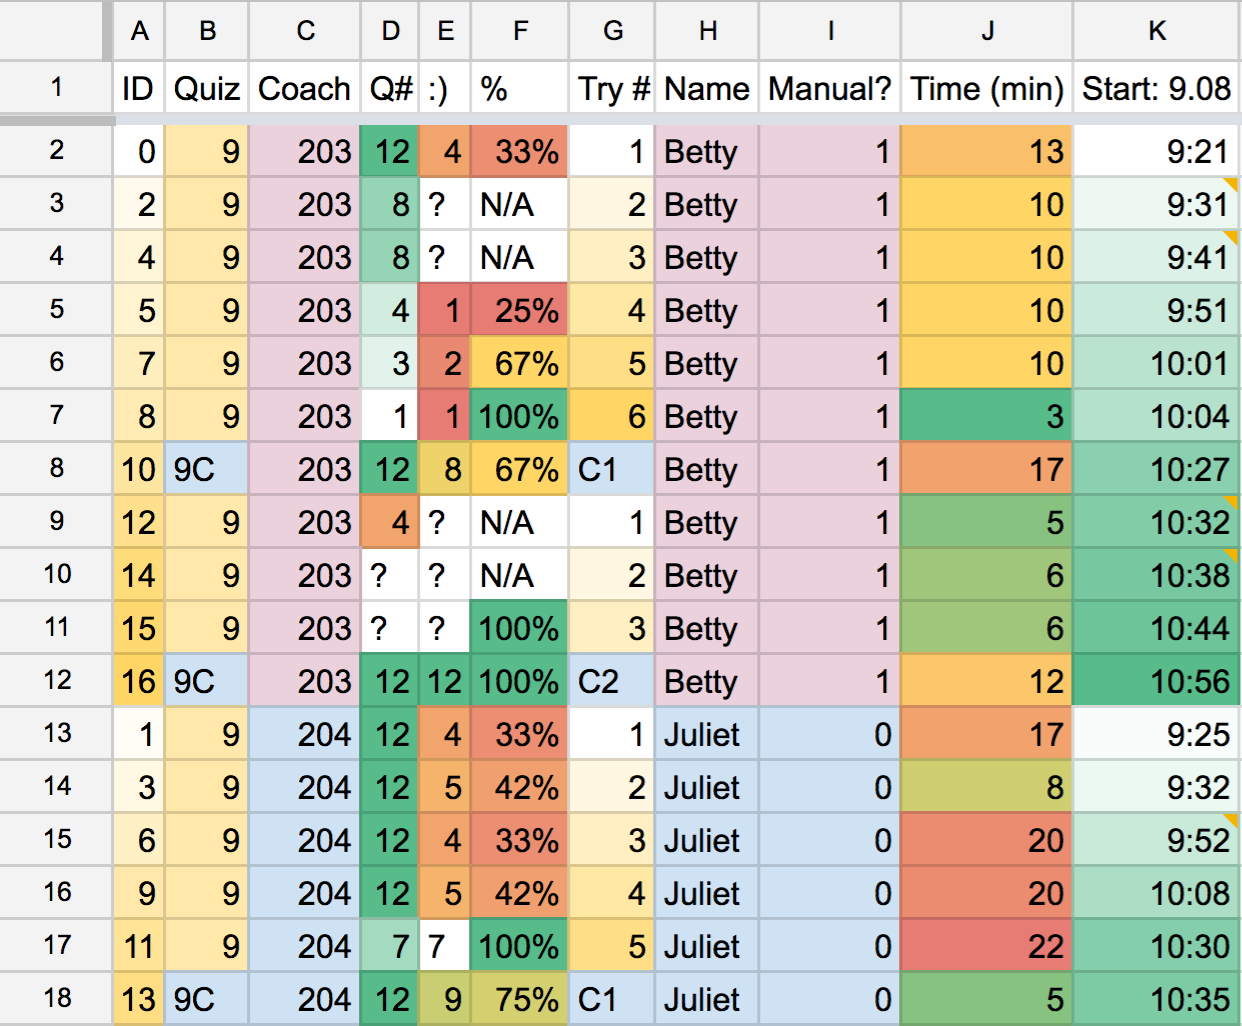
\includegraphics[width=0.8\textwidth]{analysis/areYouSureQuiz.png}
    \caption{Data analysis in Google Sheets from the quiz results during the workshop for the coach guide quiz 9: "Are you ready?".}
    \label{fig:areYouReady}
  \end{figure}

  The two coaches did 17 quizzes on quiz 9. One was allowed to use the manual (Betty, coach ID 203), while the other could only consult the feedback via the app, see figure \ref{fig:iteration-map}, D-3 and H-3.

  Apart from the quantitative quiz results, some comments were made. Betty having 4/12 correct answers on the first question, when asked from the quiz question 13 "How comfortable and ready do you feel right now to carry out session 9? (There is no right answer, just be honest with yourself!)", answered " Ready, but I probably still want to look in the coach manual and participant manual.". The other alternatives were: "Not ready at all, I need to prepare myself more by using the coach manual and participant manual.", "Somehow ready, but I still need to look more in the coach manual and participant manual." or "Very ready and comfortable.".

  Betty got 4/12 correct answers on her first try, but eventually she did pass the certification, getting 12/12 correct answers in one try in 102 minutes from the quiz start. It took her 43 minutes from her quiz try 1 to passing the training. She then failed the certification try 1 (i.e. not getting Gold) after spending 17 minutes with it. thus, she needed to go back to the training. Back in the training, now she got 8/12 instead of 4/12, and passed the whole training in 17 minutes. Then, she got 12/12 in the certification test (earning Silver), in only 12 minutes.

  Juliet also got 4/12 correct answers on her first try. Not understanding the "Improve" button, she repeatedly went back to the home screen and retook the whole test (like in iteration 2). This was a slow approach. On her new tries, she got 5/12, 4/12, 5/12, which showed that learning was too hard. Similar results had been found in iteration 1 using Duolingo, where the app failed to train the coach to get a better score. After this try, she was explained the "Try again" button, got 7/7 (spending 22 minutes with the questions compared with her 16.25 minutes average doing all 12 questions, which showed she really put effort into analyzing the answers properly). Unlocking the certification test, she got 9/12 in 5 minutes, an improvement from 4/12 on her quiz try 1 75 minutes before.

  The results from this quiz shows that:
  \begin{itemize}
  \item "Improve", only needing to repeat the questions you are not sure of, does improve learning quality and speed, compared to retaking the whole quiz again after each try - it makes learning more focused on what you need to train
  \item It needs to be clearer that you should press "Improve", for example by changing the text to "Try again"
  \item The time needed to become reliant on the session takes too long. To pass the rule of thumb for deliberate practice, a session getting to 95\% reliability should take 45-90 minutes. For Betty, it took 102 minutes from quiz start to being 100\% reliable. For Juliet, she did only manage to get 75\% reliable within the same time frame. Either scaffolding needs to increase (dividing the quiz into smaller chunks), or learning effectiveness needs to increase (for example by better feedback).
  \end{itemize}

The data and observations also shows that learning Correct Structure and Time Management via multiple-choice is not effective. Especially, this is shown by the time it takes to get a high score. To score well on such a test, the coach would retrieve from memory using a clear mental image. In its current design, getting a clear mental picture is not supported from the multiple-choice design. See Future Work in chapter \ref{future-work} for a further discussion how this Correct Structure and Time Management can be better assessed in the future.
